\normalsize
\subsection{Gravity Current Simulation - colocated Grid}
\label{chapter:NumericalTest-colocated}

The numerical model also implemented the colocated grid and is tested with the Figure 9 case\footnotemark[1] \cite{Maxworthy2002}. The resolutions are $NX \times NZ = 140 \times 60$($\Delta x = 0.01 m \Delta z = 0.0025 m$), $280 \times 120$, and $560 \times 240$. The following plots show the similarity of the two resolutions $280 \times 120$ and $560 \times 240$.

\footnotetext[1]{The salinity of the released volume in the numerical test is $\sim$ 5.5\% smaller.}

\begin{figure}[htbp]
  \begin{center}
\subfigure[$NX \times NZ = 140 \times 60$]
{
\includegraphics[width=5.2in]{../figures/colocated/Fig9case/140-60-03-VE-6/08.png}
}
\subfigure[$NX \times NZ = 280 \times 120$]
{
\includegraphics[width=5.2in]{../figures/colocated/Fig9case/280-120-0075-VE-6-Surf0/08.png}
}
\subfigure[$NX \times NZ = 560 \times 240$]
{
\includegraphics[width=5.2in]{../figures/colocated/Fig9case/560-240-00375-VE-6-Surf0/08.png}
}
\subfigure[$NX \times NZ = 560 \times 240$ of staggered grid]
{
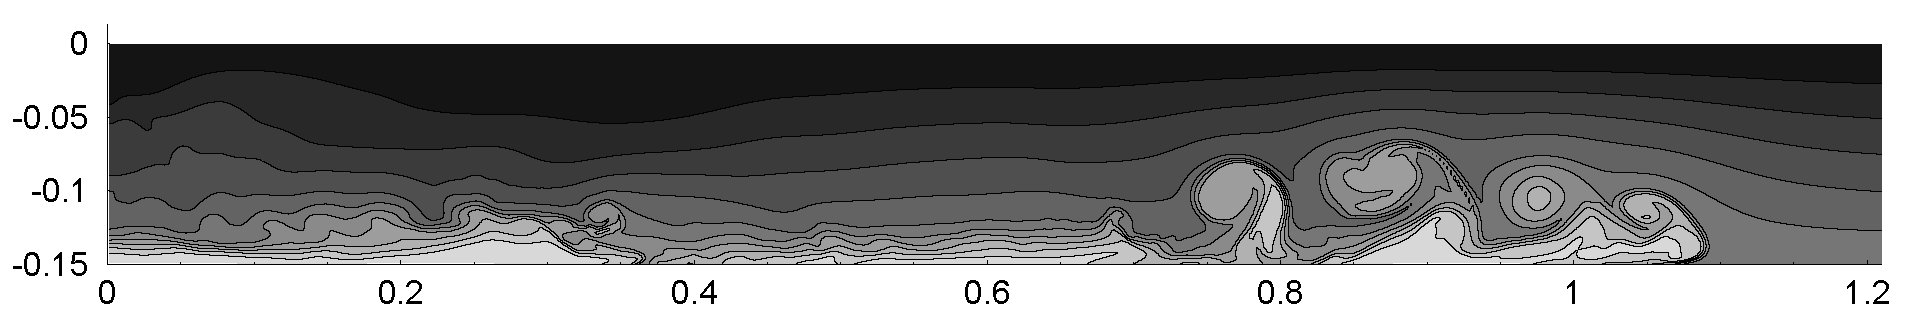
\includegraphics[width=5.2in]{../figures/Staggered/Fig9case/060526a-560-240-00375-VE-6/08.png}
}
\caption{Gravity current simulation plots at $t=6.3 (sec)$ with colocated grid of different resolutions.}
  \end{center}
\end{figure}

\cp

\normalsize
\subsection{Gravity Current Simulations - Viscosity Coefficient}
The viscosity coefficient is tested from $10^{-5} (m^2/s)$ to $10^{-7} (m^2/s)$. It shows that the gravity front propagates at a faster speed with a smaller viscosity coefficient.
\begin{figure}[htbp]
  \begin{center}
\subfigure[$\nu=10^{-5}$] % caption for subfigure b
{
\includegraphics[width=5.2in]{../figures/colocated/Fig9case/140-60-03-VE-5/08.png}
}
\subfigure[$\nu=10^{-6}$] % caption for subfigure b
{
\includegraphics[width=5.2in]{../figures/colocated/Fig9case/280-120-0075-VE-6-Surf0/08.png}
}
\subfigure[$\nu=5 \times 10^{-7}$] % caption for subfigure a
{
\includegraphics[width=5.2in]{../figures/colocated/Fig9case/280-120-0075-V5E-7-Surf0/08.png}
}
\subfigure[$\nu=10^{-7}$] % caption for subfigure b
{
\includegraphics[width=5.2in]{../figures/colocated/Fig9case/280-120-0075-VE-7-Surf0/08.png}
}
\caption{Gravity current simulation plots at $t=6.3 (sec)$ with colocated grid  and Strong-Stability- Preserving Runge-Kutta time integration scheme.}
  \end{center}
\end{figure}


\cp

